









\formatChapter{Pink Tag Boulders}

\raggedcolumns
\begin{multicols}{2}

\qrcode{./maps/qr//Pink Tag Boulders_qr.png}{http://maps.google.com/maps?q=44.43998124232581,-122.57539325959186}{Navigate to this area}
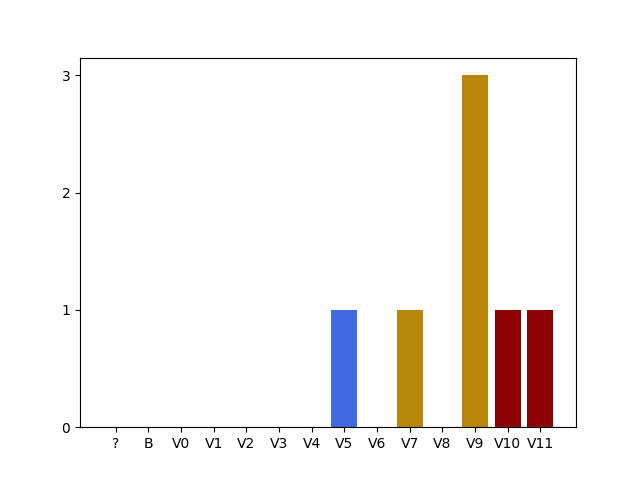
\includegraphics[width=0.9\linewidth]{./maps/plots//Pink Tag Boulders.png}
\end{multicols}
\begin{multicols}{2}
Just across the road from the main area lay a few boulders on the banks of the River. Beware the water level can rise quickly blocking off access to some of the boulders in this area. Consult the USGS flow charts for below green peter damn to know when the river will be low. See driving directions for the Garden Main area.\\

\textbf{NOTE: This area is mostly incomplete. Look forward to more information in future revisions of this book or contribute your own knowledge on github.}\\


\newpage






\end{multicols}
\clearpage